\documentclass{article}
\usepackage{pgfplots}
\pgfplotsset{width=10cm,compat=1.9}

\begin{document}

\title{Analysis of Cat-Dog Classification Models}
\author{Tugay Talha İçen}
\date{October, 2023}

\maketitle0

\section{Introduction}
In this report, I present the performance metrics of several VGG model architectures for a cat-dog classification task, including the effect of Image Data Augmentation (IDA) and different learning rates. Each model is assessed based on its training time and classification accuracy. The models vary based on the number of blocks they contain, ranging from one to seven, and whether they include dropout layers or IDA.

\section{Models and Training}
The models consist of convolutional neural network architectures based on VGG, with blocks varying from one to seven. Each block contains a 2D convolution layer followed by a max pooling layer. The dropout models additionally have dropout layers included after each max pooling operation for regularization. Some models have also incorporated IDA. Finally, I also varied the learning rate in some models to observe its effect on performance and learning time.

\section{Results}

\textbf{M1}: 1 blocks \& 4 layers VGG model 
\textbf{M2}: 2 block \& 5 layers VGG model
\\\textbf{M3}: 3 block \& 6 layers VGG model 
\textbf{M4}: 4 block \& 7 layers VGG model
\\\textbf{M5}: 5 block \& 8 layers VGG model 
\textbf{M6}: 7 block \& 10 layers VGG model
\\\textbf{Dropout 1}: M1 model with dropout regularization. 
\\\textbf{Dropout 2}: M2 model with dropout regularization.
\\\textbf{Dropout 3}: M3 model with dropout regularization. 
\\\textbf{Dropout 4}: M4 model with dropout regularization.
\\\textbf{Dropout 5}: M5 model with dropout regularization. 
\\\textbf{Dropout 6}: M6 model with dropout regularization.
\\\textbf{IDA Model}: M3 model with Image Data Augmentation.
\\\textbf{Dropout IDA Model}: Dropout 3 model with Image Data Augmentation.
\\\textbf{Dropout (LR=X)}: Dropout 3 model with learning rate X.
\\\textbf{Batch Size: X (X= Batch size)}: M6 model with batch size X.
\\20 epochs are used for normal models, 50 epochs are used for dropout models and 100 epochs are used for IDA models and learning rate test models.

The following table lists the training time and accuracy for each model:

\begin{table}[h!]
\begin{center}
\begin{tabular}{|c|c|c|}
\hline
Model & Training Time (seconds) & Accuracy (\%)\\
\hline
M1 & 1053.07 & 69.475\\
M2 & 1096.75 & 76.059\\
M3 & 1162.90 & 80.216\\
M4 & 1113.49 & 81.707\\
M5 & 1113.34 & 81.818\\
M6 & 1187.38 & 82.342\\
Dropout 1 & 2341.55 & 72.997\\
Dropout 2 & 2576.91 & 78.026\\
Dropout 3 & 2721.81 & 81.945\\
Dropout 4 & 2722.27 & 80.105\\
Dropout 5 & 2763.94 & 81.707\\
Dropout 6 & 2980.78 & 78.486\\
Dropout 6 (100 epochs) & 7053.15 & 91.179\\
IDA Model & 14849.57 & 87.815\\
Dropout IDA Model & 14160.34 & 88.101\\
Dropout (LR=0.0001) & 4867.64 & 73.727\\
Dropout (LR=0.0010) & 5358.49 & 82.865\\
Dropout (LR=0.0030) & 8024.23 & 84.515\\
Dropout (LR=0.0100) & 8587.45 & 84.214\\
Dropout (LR=0.0300) & 5083.72 & 49.595\\
Batch Size: 8 & 1285.326 & 0.947 \\
Batch Size: 16 & 1041.039 & 0.926 \\
Batch Size: 32 & 920.357 & 0.921 \\
Batch Size: 64 & 873.642 & 0.904 \\
Batch Size: 128 & 861.372 & 0.893 \\
Batch Size: 256 & 850.574 & 0.876 \\
\hline
\end{tabular}
\end{center}
\caption{Training time and accuracy for each model, including the results from varying batch sizes.}
\end{table}


% First Chart: Normal Models
\begin{center}
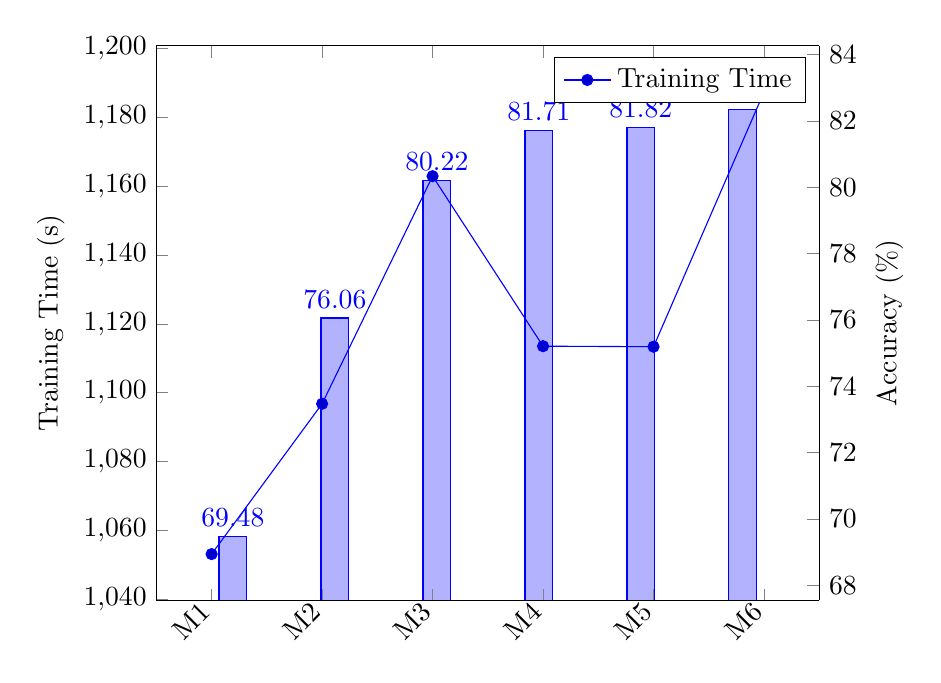
\begin{tikzpicture}
\begin{axis}[
  axis y line*=right,
  axis x line=none,
  ylabel={Accuracy (\%)},
  symbolic x coords={M1,M2,M3,M4,M5,M6},
  xtick=data,
  nodes near coords,
  nodes near coords align={vertical},
  ybar,
  enlargelimits=0.15,
]
\addplot coordinates {(M1,69.475) (M2,76.059) (M3,80.216) (M4,81.707) (M5,81.818) (M6,82.342)};
\legend{Accuracy}
\end{axis}
\begin{axis}[
    axis y line*=left,
    ylabel={Training Time (s)},
    symbolic x coords={M1,M2,M3,M4,M5,M6},
    xtick=data,
    x tick label style={rotate=45,anchor=east},
    ]
\addplot+[sharp plot, color=blue] coordinates {(M1,1053.07) (M2,1096.75) (M3,1162.90) (M4,1113.49) (M5,1113.34) (M6,1187.38)};
\legend{Training Time}
\end{axis}
\end{tikzpicture}
\end{center}

% Second Chart: Dropout Models
\begin{center}
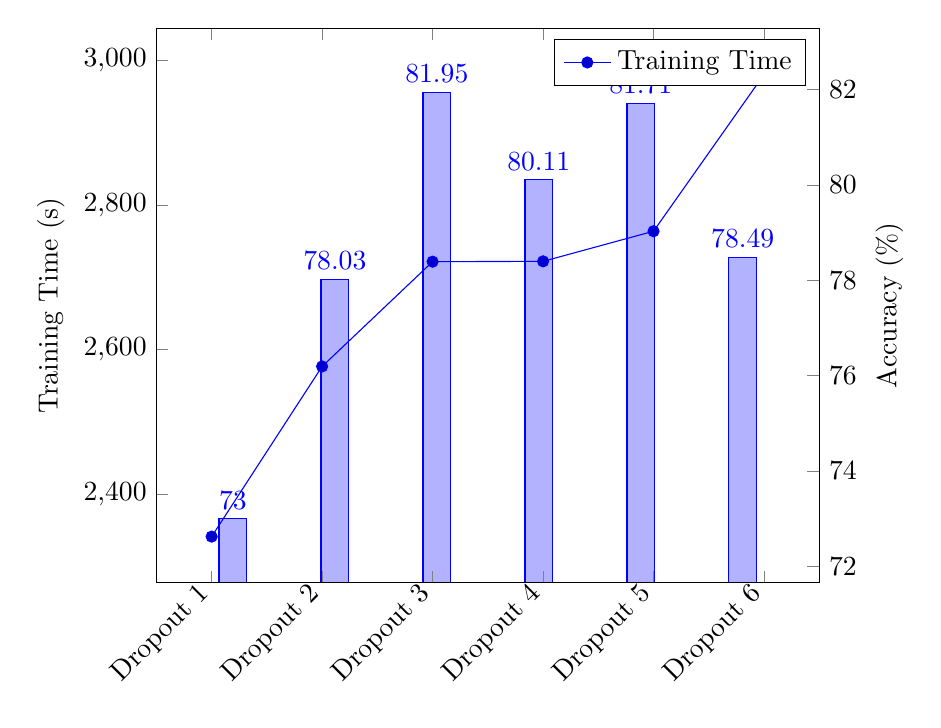
\begin{tikzpicture}
\begin{axis}[
  axis y line*=right,
  axis x line=none,
  ylabel={Accuracy (\%)},
  symbolic x coords={Dropout 1,Dropout 2,Dropout 3,Dropout 4,Dropout 5,Dropout 6},
  xtick=data,
  nodes near coords,
  nodes near coords align={vertical},
  ybar,
  enlargelimits=0.15,
]
\addplot coordinates {(Dropout 1,72.997) (Dropout 2,78.026) (Dropout 3,81.945) (Dropout 4,80.105) (Dropout 5,81.707) (Dropout 6,78.486)};
\legend{Accuracy}
\end{axis}
\begin{axis}[
    axis y line*=left,
    ylabel={Training Time (s)},
    symbolic x coords={Dropout 1,Dropout 2,Dropout 3,Dropout 4,Dropout 5,Dropout 6},
    xtick=data,
    x tick label style={rotate=45,anchor=east},
    ]
\addplot+[sharp plot, color=blue] coordinates {(Dropout 1,2341.55) (Dropout 2,2576.91) (Dropout 3,2721.81) (Dropout 4,2722.27) (Dropout 5,2763.94) (Dropout 6,2980.78)};
\legend{Training Time}
\end{axis}
\end{tikzpicture}
\end{center}

% Third Chart: M6 and its variations
\begin{center}
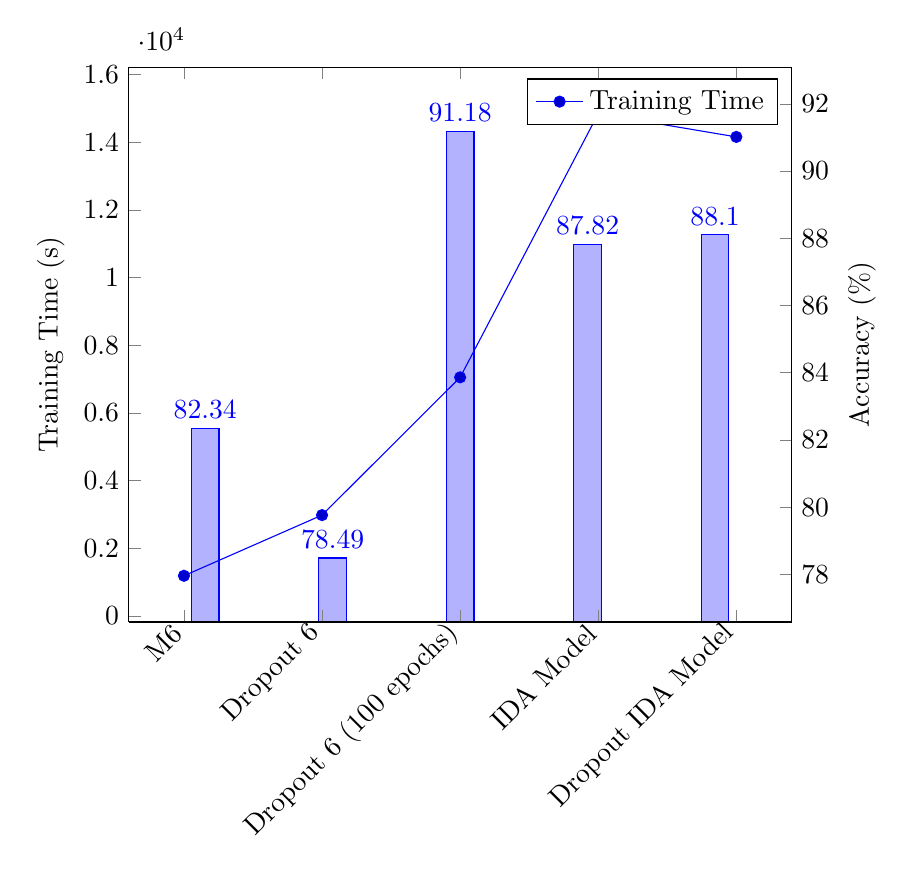
\begin{tikzpicture}
\begin{axis}[
  axis y line*=right,
  axis x line=none,
  ylabel={Accuracy (\%)},
  symbolic x coords={M6,Dropout 6,Dropout 6 (100 epochs), IDA Model, Dropout IDA Model},
  xtick=data,
  nodes near coords,
  nodes near coords align={vertical},
  ybar,
  enlargelimits=0.15,
]
\addplot coordinates {(M6,82.342) (Dropout 6,78.486) (Dropout 6 (100 epochs),91.179) (IDA Model,87.815) (Dropout IDA Model,88.101)};
\legend{Accuracy}
\end{axis}
\begin{axis}[
    axis y line*=left,
    ylabel={Training Time (s)},
    symbolic x coords={M6,Dropout 6,Dropout 6 (100 epochs), IDA Model, Dropout IDA Model},
    xtick=data,
    x tick label style={rotate=45,anchor=east},
    ]
\addplot+[sharp plot, color=blue] coordinates {(M6,1187.38) (Dropout 6,2980.78) (Dropout 6 (100 epochs),7053.15) (IDA Model,14849.57) (Dropout IDA Model,14160.34)};
\legend{Training Time}
\end{axis}
\end{tikzpicture}
\end{center}

\begin{center}
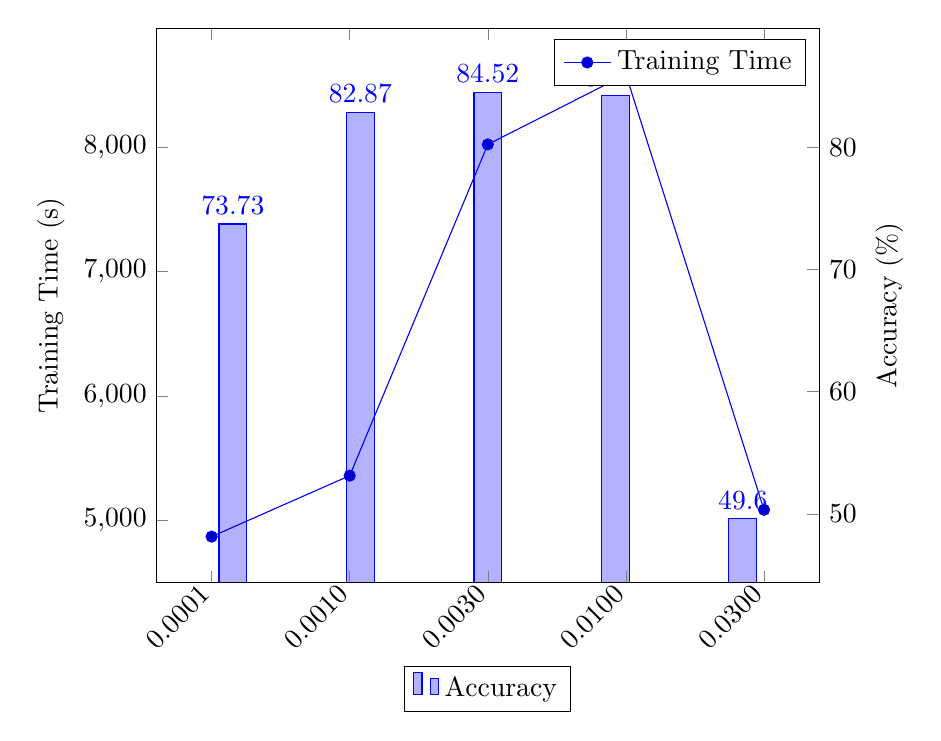
\begin{tikzpicture}
\begin{axis}[
  axis y line*=right,
  axis x line=none,
  ylabel={Accuracy (\%)},
  symbolic x coords={0.0001,0.0010,0.0030,0.0100,0.0300},
  xtick=data,
  nodes near coords,
  nodes near coords align={vertical},
  ybar,
  enlargelimits=0.15,
  legend style={at={(0.5,-0.15)},
  anchor=north,legend columns=-1},
]
\addplot coordinates {(0.0001,73.727) (0.0010,82.865) (0.0030,84.515) (0.0100,84.214) (0.0300,49.595)};
\legend{Accuracy}
\end{axis}
\begin{axis}[
    axis y line*=left,
    ylabel={Training Time (s)},
    symbolic x coords={0.0001,0.0010,0.0030,0.0100,0.0300},
    xtick=data,
    x tick label style={rotate=45,anchor=east},
    ]
\addplot+[sharp plot, color=blue] coordinates {(0.0001,4867.64) (0.0010,5358.49) (0.0030,8024.23) (0.0100,8587.45) (0.0300,5083.72)};
\legend{Training Time}
\end{axis}
\end{tikzpicture}
\end{center}


% Visual Representation for Batch Sizes
\begin{center}
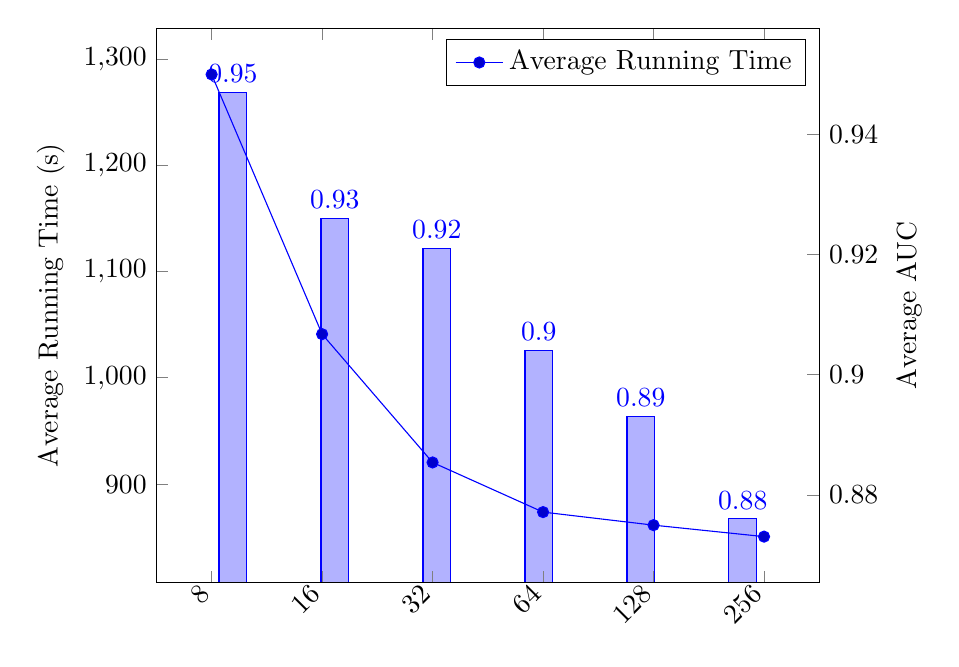
\begin{tikzpicture}
\begin{axis}[
  axis y line*=right,
  axis x line=none,
  ylabel={Average AUC},
  symbolic x coords={8,16,32,64,128,256},
  xtick=data,
  nodes near coords,
  nodes near coords align={vertical},
  ybar,
  enlargelimits=0.15,
]
\addplot coordinates {(8,0.947) (16,0.926) (32,0.921) (64,0.904) (128,0.893) (256,0.876)};
\legend{Average AUC}
\end{axis}
\begin{axis}[
    axis y line*=left,
    ylabel={Average Running Time (s)},
    symbolic x coords={8,16,32,64,128,256},
    xtick=data,
    x tick label style={rotate=45,anchor=east},
    ]
\addplot+[sharp plot, color=blue] coordinates {(8,1285.326) (16,1041.039) (32,920.357) (64,873.642) (128,861.372) (256,850.574)};
\legend{Average Running Time}
\end{axis}
\end{tikzpicture}
\end{center}



\section{Conclusion}
This report presents results from a cat-dog classification task using several VGG-based models, including variations in the number of blocks, dropout regularization, Image Data Augmentation (IDA), different learning rates, and the effects of different batch sizes.
\\  The results demonstrate how these factors affect training time and model accuracy. In general, models with dropout layers and IDA have higher training times due to the increased complexity and the additional data generated for training. The highest accuracy was achieved by the dropout 6 model with 100 epochs. In addition to that by looking at the tests on the 3-layer model, we can say that the image data augmentation models significantly increase the performance, and if I applied it on the dropout 6 model, we could achieve much better results(It didn't due to length of training times). Variations in batch sizes also influenced training times and accuracies; notably, smaller batch sizes, although more computationally intensive, resulted in higher Average AUC scores. About the learning rates, their performance can be better interpreted by looking at the graphs inside the results folder and when we look at that graphs the the fastest and most consistent learning rate for our model is 0.01 lower lrs than that are slower and 0.03 is not learning successfully. 


\end{document}
